\documentclass[a4paper, 12pt, addpoints]{exam}
\usepackage{IfbaListas}
%==============================================================
\NumList{4} %NÚMERO DA LISTA
\Assunto{Conjuntos}
%==============================================================
%=========================================================
%------------Cabeçalho e rodapé 
%=========================================================
\pagestyle{headandfoot}%{head}%empty
\firstpageheader{}{}{}
\runningheader{\disciplina}{}{Lista \numlist: \assunto}
\runningheadrule
% \copyright \professor
\firstpagefooter{}{}{Pag. \thepage\ de \numpages}
%\iflastpage{Outros templates em \href{http://gg.gg/profwaldexsantos}{gg.gg/profwaldexsantos}
\runningfooter{}{}{Pag. \thepage\ de \numpages}
\runningfootrule
%===============================================================
%INFORMAÇÕES SOBRE A AVALIAÇÃO
\nomeInst{Instituto Federal da Piauí}
\logoInst{
\includegraphics[scale=0.17]{Figs/IFPIPicosVertical.png}}
\Campus{Picos} %PARA ENSINO FUNDAMENTAL OU MÉDIO-COMENTE ESTA LINHA COM %
\nomeCurso{Análise e Desenvolvimento de Sistemas} %Se não for curso superior, basta comentar esta linha ou deixar em branco
\nomeDisciplina{Matemática Computacional}
\Semestre{1}
\nomeProfessor{Rogerio Figueredo de Sousa}
\Aluno{}
\matriculaAluno{}
%===============================================================
 %CARREGA AS INFORMAÇÕES GERAIS DO PROFESSOR, ESCOLA ETC
%==============================================================

%COMEÇO DO DOCUMENTO
\begin{document}
\info\vspace{-1 cm} %Imprime as informações do cabeçalho programada no pacote 
% inicia a gravacao da resposta no arquivo "ans" cujo nome externo é gabarito 
\Opensolutionfile{ans}[Gabarito]
%*****************************************************************************
\begin{questions}%COMEÇA O AMBIENTE DE QUESTÕES
  \question Julgue se os conjuntos são finitos ou infinitos:
  \begin{enumerate}[a)]
    \item Conjunto das letras do alfabeto;
    \item $P = \{y | y = 2x ~ e ~ x \in \mathbb{N} \}$
    \item $M = \{x \in \mathbb{N} | x > 0 ~ e ~ x < 6\}$
    \item O conjunto do números naturais.
\end{enumerate}  
  
    \begin{resp}~
        \begin{multicols}{4}
        \begin{enumerate}[a)]
            \item Finito
            \item Infinito
            \item Finito
            \item Infinito
        \end{enumerate}
    \end{multicols}
    
    \end{resp}

  \question Descreva cada um dos conjuntos a seguir listando seus elementos:

  \begin{multicols}{2}
    \begin{enumerate}
      \item $A=\{x|x ~ \acute{e} ~ um ~ inteiro ~ e ~ 3 < x < 8\}$
      \item $B=\{x|x ~ \acute{e} ~ um ~ m\hat{e}s ~ com ~ exatamente ~ 30 ~ dias\}$
      \item $C=\{x|x ~ \acute{e} ~ a ~ capital ~ do ~ Brasil\}$
      \item $D=\{x|(\exists y)(y \in \{0,1,2\} ~ e ~ x = y^3)\}$
      \item $E=\{x|x \in \mathbb{N} ~ e ~ (\exists y)(y \in \mathbb{N} ~ e ~ x \leq y)\}$
      \item $F=\{x|x \in \mathbb{N} ~ e ~ (\forall y)(y \in \mathbb{N} ~ \rightarrow ~ x \leq y)\}$
      \item $A = \{x | x \in \mathbb{N} ~ e ~ (\forall y)(y \in \{2, 3, 4, 5\}) \rightarrow x \geq y\}.$
      \item $B = \{x | (\exists y)(\exists z)(y \in \{1,2\} ~ e ~ z \in \{2,3\} ~ e ~ x=y+z)\}$
  \end{enumerate}    
  \end{multicols}

  \begin{resp}~
    \begin{multicols}{2}
    \begin{enumerate}[a)]
        \item $A = \{ 4, 5, 6, 7\}$
        \item $B = \{ Abril, Junho, Setembro, Novembro \}$
        \item $C = \{Bras\acute{i}lia\}$
        \item $D = \{ 0, 1, 8\}$
        \item $E = \{0, 1, 2, ...\}$
        \item $F = \{ 0 \}$
        \item $A = \{ 5, 6, 7, ...\}$
        \item $B = \{ 3, 4, 5\}$
    \end{enumerate}
\end{multicols}

\end{resp}

  \question Descreva cada um dos conjuntos a seguir através de uma relação de recorrência.

  \begin{enumerate}[a)]
    \item $A=\{2,4,16,256,...\}$
    \item $B=\{1,4,9,16,...\}$
    \item $C=\{1,3,9,27,...\}$
\end{enumerate} 

\begin{resp}~

    \begin{enumerate}[a)]
        \item
            
        \begin{itemize}
                \item $2 \in A$
                \item Se $n \in A$, então $n^2 \in A$
            \end{itemize}

        \item 
            
            \begin{itemize}
                    \item $a_1 = 1$
                    \item $n \in \mathbb{N+}, a_{n+1} = a_{n} + 2n - 1$
                \end{itemize}

        \item 
            
        \begin{itemize}
                \item $1 \in C$
                \item Se $n \in C$, então $3n \in C$
            \end{itemize}
    \end{enumerate}
\end{resp}
  
\question Sejam $A = \{x | x \in \mathbb{N} ~ e ~ x \geq 5\}$, $B = \{10, 12, 16, 20\}$ e $C = \{x | (\exists y)(y \in \mathbb{N} ~ e ~ x = 2y)\}$

Quais das proposições abaixo são verdadeiras:

\begin{multicols}{2}
  \begin{enumerate}[a)]
      \item $B \subseteq C$
      \item $B \subset A$
      \item $A \subseteq C$
      \item $26 \in C$
      \item $\{11, 12, 13\} \subseteq A$
      \item $\{11, 12, 13\} \subset C$
      \item $\{12\} \in B$
      \item $\{12\} \subseteq B$
      \item $\{x | x \in \mathbb{N} ~ e ~ x < 20\} \nsubseteq B$
      \item $5 \subseteq A$
      \item $\{\emptyset\} \subseteq B$
      \item $\emptyset \notin A$
  \end{enumerate}
\end{multicols}

\begin{resp}~

    \begin{multicols}{4}
        \begin{enumerate}[a)]
            \item V
            \item V
            \item F
            \item V
            \item V
            \item F
            \item F (Operador $\in$ é aplicado a elementos e não a conjuntos)
            \item V
            \item V
            \item F (observar operador)
            \item F
            \item V
        \end{enumerate}
      \end{multicols}
\end{resp}

\question  Sejam: $A = \{x | x \in \mathbb{R} ~ e ~ x^2 - 4x + 3 = 0\}$
 e $B = \{x | x \in \mathbb{N} ~ e ~ 1 \leq x \leq 4\}$
\vspace{4mm}
Prove que $A \subset B.$

\begin{resp}~
    
    Seja $x \in A$. Então $x \in \mathbb{R}$ e $x^2 - 4x + 3 = 0$ ou $(x - 1)(x - 3) = 0$, o que nos dá $x = 1$ ou $x = 3$. Em qualquer dos casos, $x \in \mathbb{N}$ e $1 \leq x \leq 4$, de modo que $x \in B$. Portanto, $A \subseteq B$. O número 4 pertence a B, mas não pertence a A, logo $A \subset B$.
\end{resp}


\question Sejam $ A = \{x|x \in \mathbb{N} ~ e ~ x^2 < 15\} $
e $ B = \{x|x \in \mathbb{N} ~ e ~ 2x < 7 \} $

Prove que $A = B.$

\begin{resp}~
    
    Sejam $A = \{x | x \in x^2 < 15\}$ e $B = {x | x \in \mathbb{N} e 2x < 7}$.
    
    Para provar que $A = B$, vamos mostrar que $A \subseteq B$ e $B \subseteq A$. Para $A \subseteq B$, precisamos escolher um elemento arbitrário de A — ou seja, qualquer coisa que satisfaça a propriedade que caracteriza os elementos de A — e mostrar que satisfaz a propriedade que caracteriza os elementos de B. Seja $x \in A$. Então $x$ é um inteiro não negativo que satisfaz a desigualdade $x^2 < 15$. Os inteiros não negativos cujos quadrados são menores do que 15 são 0, 1, 2 e 3, logo esses são os elementos de A. O dobro de cada um desses inteiros não negativos é um número menor do que 7. Portanto, todo elemento de A pertence a B e $A \subseteq B$.

    Vamos mostrar agora que $B \subseteq A$. Todo elemento de B é um inteiro não negativo cujo dobro é menor do que 7. Esses números são 0, 1, 2 e 3, e cada um deles tem o quadrado menor do que 15, logo $B \subseteq A$.
\end{resp}

\question Para $A=\{1,2,3\}$, qual é o $\wp(A)$?

\begin{resp}~
    
    $\wp(A) = \{\emptyset, \{1\}, \{2\}, \{3\}, \{1, 2\}, \{1, 3\}, \{2, 3\}, \{1, 2, 3\}\}$.
\end{resp}

\question Se S tem \textit{n} elementos, então $\wp(A)$ tem quantos elementos?


\begin{resp}~

    $2^n$ elementos.
\end{resp}


\question Sobre o conjunto $A = \{1, 2, 3, 4\}$, considere as afirmativas a seguir.

\begin{enumerate}
    \item $\mathcal{P}(A) = \{\emptyset, \{2, 3, 4\}\}$ é uma partição de $A$.
    \item $\mathcal{P}(A) = \{\emptyset, \{1, 2, 3\}, \{3, 4\}\}$ é uma partição de $A$.
    \item $\mathcal{P}(A) = \{\{1, 2\}, \{3, 4\}\}$ é uma partição de $A$.
    \item $\mathcal{P}(A) = \{\{1\}, \{2\}, \{3\}, \{4\}\}$ é uma partição de $A$.
\end{enumerate}



\noindent
Assinale a alternativa correta.

\begin{enumerate}[a)]
    \item Somente as afirmativas I e II são corretas;
    \item Somente as afirmativas I e IV são corretas;
    \item Somente as afirmativas III e IV são corretas;
    \item Somente as afirmativas I, II e III são corretas;
    \item Somente as afirmativas II, III e IV são corretas;
\end{enumerate}

\begin{resp}~
    
    c
\end{resp}

\question Sejam
\[ A = \{x | x ~ \acute{e} ~ um ~ inteiro ~ n\tilde{a}o - negativo ~ par \} \]
\[ B = \{x | (\exists y) (y \in \mathbb{N} ~ e ~ x = 2y + 1 )\} \]
\[ C = \{x|(\exists y)(y \in \mathbb{N} ~ e ~ x = 4y)\} \]

Julgue a veracidade de cada alternativa:

\begin{enumerate}[a)]
    \item $A \cup B$
    \item $A = B$
    \item $ C \subset A$
    \item $A \cup C$
    \item $A - C = \{x|(\exists y)(y \in \mathbb{N} ~ e ~ x = 4y + 2)\}$
\end{enumerate}

\begin{resp}~
    
    \begin{multicols}{2}
    \begin{enumerate}[a)]
        \item - (anulada) [$A \cup B = \mathbb{N}$]
        \item F
        \item V
        \item - (anulada) [$A \cup C = A$]
        \item V
    \end{enumerate}
\end{multicols}
\end{resp}

\question Sejam
\[ A = \{1,2,3,5,10\} \]
\[ B = \{2,4,7,8,9\} \]
\[ C = \{5,8,10\} \]

Se $S=\{1,2,3,4,5,6,7,8,9,10\}$, encontre:

\begin{enumerate}[a)]   
    \item $|A| + |B|$
    \item $A \cup B$
    \item $A - C$
    \item $B \cap (A \cup C)$
    \item $\overline{C}$
\end{enumerate}

\begin{resp}~
    
    \begin{multicols}{2}
    \begin{enumerate}[a)]   
        \item 10
        \item $\{1,2,3,4,5,7,8,9,10\}$
        \item $\{ 1,2,3 \}$
        \item $\{ 2,8 \}$
        \item $\{ 1,2,3,4,6,7,9 \}$
    \end{enumerate}
\end{multicols}
\end{resp}

\question Usando as identidades básicas, prove a identidade:

\[
[C \cap (A \cup B)] \cup \left[(A \cup B) \cap \overline{C}\right] = A \cup B
\]

\begin{center}
    (A, B e C são subconjuntos arbitrários de $S$.)
\end{center}

\begin{resp}~
    
    \begin{multicols}{2}
        \begin{itemize}
            \item $[(A \cup B) \cap C] \cup \left[(A \cup B) \cap \overline{C} \right]$
            \item $(A \cup B) \cap (C \cup \overline{C})$
            \item $(A \cup B) \cap S$
            \item $(A \cup B)$
        \end{itemize}

        \begin{itemize}
            \item (comutatividade)
            \item (distributividade)
            \item (complemento)
            \item (elemento neutro)
        \end{itemize}
    \end{multicols}
\end{resp}

\question Enuncie a identidade dual do exemplo anterior.

\begin{resp}~

    $[C \cup (A \cap B)] \cap \left[(A \cap B) \cup \overline{C}\right] = A \cap B$
    
\end{resp}

\question Usando as identidades básicas, prove a identidade: 
        
\[
(A \cup B) \cap (A \cup \overline{B}) = A
\]

\begin{resp}~
    
    \begin{multicols}{2}
        \begin{itemize}
            \item $A \cup (B \cap \overline{B})$
            \item $A \cup \emptyset$
            \item $A$
        \end{itemize}

        \begin{itemize}
            \item (distributividade)
            \item (complemento)
            \item (elemento neutro)
        \end{itemize}
    \end{multicols}
\end{resp}


\question Liste os elementos dos seguintes conjuntos:
\begin{enumerate}[a)]
    \item $\{ x ~ | ~ x ~ \acute{e} ~ um ~ n\acute{u}mero ~ real ~ e ~ x^2 = 1 \}$
    \item $\{ x ~ | ~ x \in \mathbb{Z} ~ e ~ |x| < 4 \}$ ($|x|$ denota a função valor absoluto)
    \item $\{x ~ | ~ x ~ \acute{e} ~ m\acute{u}ltiplo ~ de ~ 4 \}$
\end{enumerate}

\begin{resp}~
    \begin{enumerate}[a)]
        \item $\{ -1, 1 \}$
        \item $\{ -3, -2, -1, 0, 1, 2, 3 \}$ 
        \item $\{{4,8,12,16,20,...} \}$
    \end{enumerate}
    
\end{resp}

\question Descreva cada um dos seguintes conjuntos, atribuindo-lhes uma propriedade específica:
\begin{enumerate}[a)]
    \item $S = \{1, 4, 9, 16\}$
    \item $S = \{2, 3, 5, 7, 11, 13, . . . \}$
    \item $S = \{0, 1, 10, 11, 100, 101, 110, 111, 1000, \dots \}$
\end{enumerate}

\begin{resp}~

    \begin{enumerate}[a)]
        \item $\{ x | (\exists y)( y \in \{1,2,3,4\} ~ e ~ x = y^2) \}$
        \item $\{ x | \text{x são os números primos}\}$ 
        \item $\{{x| \text{x é um inteiro não negativo escrito em forma binária}}\}$
    \end{enumerate}
    
\end{resp}

\question Sejam os conjuntos: $A = \{x ~ | ~ x ~ \acute{e} ~ par ~ positivo ~ e ~ x < 15\}$, $B = \{x \in N ~ | ~ x < 15\}$ e $C = \{x ~ | ~ x < 15 ~ e ~ x ~ \acute{e} ~ primo \}$. Insira os elementos correspondentes no diagrama de Euler-Venn:

\begin{resp}~

    \begin{center}
        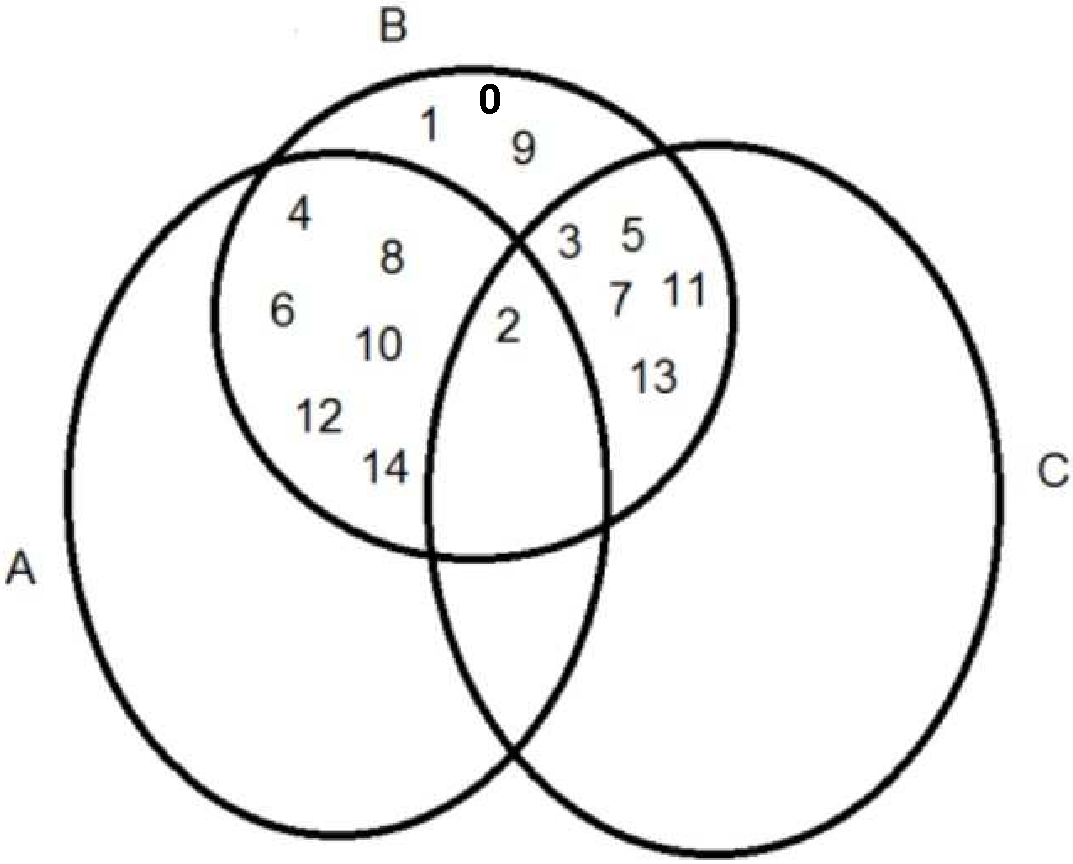
\includegraphics[width=.4\linewidth]{Figs/conjuntos-cropped.pdf}
    \end{center}
    
\end{resp}


\question Faça um diagrama de Euler-Venn que simbolize a seguinte situação: A, B, C, D são conjuntos não vazios e $D \subset C \subset B \subset A$.

\begin{resp}~
    
    \begin{center}
        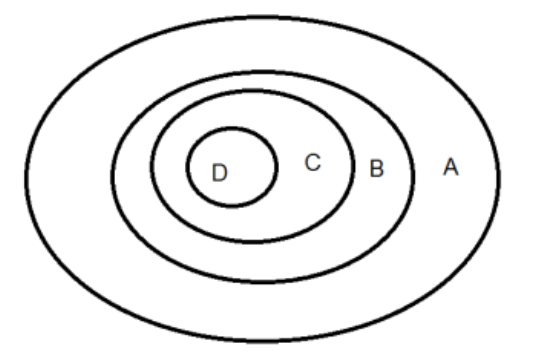
\includegraphics[width=.4\linewidth]{Figs/conjuntos2.png}
    \end{center}
\end{resp}

\question Sejam $U ~ (universo) ~ = ~ \{n \in \mathbb{N} ~ | ~ 0 \leq n \leq 9\}$, $A = \{1, 2, 3, 4\}$, $B = \{x ~ \in ~ \mathbb{R} | (x - 1) (x - 3)^3 = 0\}$ e $C = \{n ~ \in ~ \mathbb{N} | ~ n ~ \acute{e} ~ \acute{i}mpar \}$. Determine:
\begin{enumerate}[a)]
    \item $A \cup B$
    \item $A \cap (B \cup C)$
    \item $C - A$
    \item $ \overline{A} \cup C$
    \item a cardinalidade de A, B e C
\end{enumerate}

\begin{resp}~

    \begin{multicols}{2}
    \begin{enumerate}[a)]
        \item $\{1,2,3,4,5\}$
        \item $\{1,3\}$
        \item $\{5,7,9,11,...\}$
        \item $\{0,5,6,7,8,9,11,13,15,17,...\}$
        \item $\{ 4, 2, \infty\}$
    \end{enumerate}
\end{multicols}
    
\end{resp}

\question Sejam os conjuntos $A = \{a, b, c\}$, $B = \{x, y\}$ e $C = \{0, 1\}$. Encontre os seguintes produtos cartesianos:
\begin{itemize}[a)]
    \item $A \times B$
    \item $C \times A$
\end{itemize}

\begin{resp}~
    
    \begin{enumerate}[a)]
        \item $\{(a,x),(a,y),(b,x),(b,y),(c,x),(c,y)\}$
        \item $\{(0,a),(0,b),(0,c),(1,a),(1,b),(1,c)\}$
    \end{enumerate}
\end{resp}

\question A, B e C são subconjuntos de um conjunto S. Prove as identidades a seguir usando as identidades básicas envolvendo conjuntos.
\begin{enumerate}[a)]
    \item $(A \cup B) \cap (A \cup \overline{B}) = A$
    \item $A \cap (B \cap \overline{A}) = B \cap A$ [OBS: Corrigida no gabarito]
\end{enumerate}

\begin{resp}~
    
    \begin{enumerate}[a)]
    \item 
    \begin{multicols}{2}
        \begin{itemize}
            \item $A \cup (B \cap \overline{B})$
            \item $A \cup \emptyset$
            \item $A$
        \end{itemize}

        \begin{itemize}
            \item (distributividade)
            \item (complemento)
            \item (elemento neutro)
        \end{itemize}
    \end{multicols}

    \item 
    
    Correção: $A \cap (B \cup \overline{A}) = B \cap A$
    
    \begin{multicols}{2}
        \begin{itemize}
            \item $(A \cap B) \cup (A \cap \overline{A})$
            \item $(A \cap B) \cup \emptyset$
            \item $(A \cap B)$
            \item $(B \cap A)$
        \end{itemize}

        \begin{itemize}
            \item (distributividade)
            \item (complemento)
            \item (elemento neutro)
            \item (comutatividade)
        \end{itemize}
    \end{multicols}
\end{enumerate}
\end{resp}


\question Encontre A e B, se $A - B = \{1, 5, 7, 8\}$, $B - A = \{2, 10\}$, e $A \cap B = \{3, 6, 9\}$.

\begin{resp}~
    
    $A=\{1,3,5,6,7,8,9\}$ e $B=\{2,3,6,9,10\}$
\end{resp}

\question Dados os conjuntos $A = \{1, 2, 3, 4, 5\}$, $B = \{1, 2, 4, 6, 8\}$ e $C = \{2, 4, 5, 7\}$, obtenha um conjunto X tal que $X \subset A$ e $A - X = B \cap C$.

\begin{resp}~
    
    $X=\{1,3,5\}$
\end{resp}


\question 

\begin{figure}
  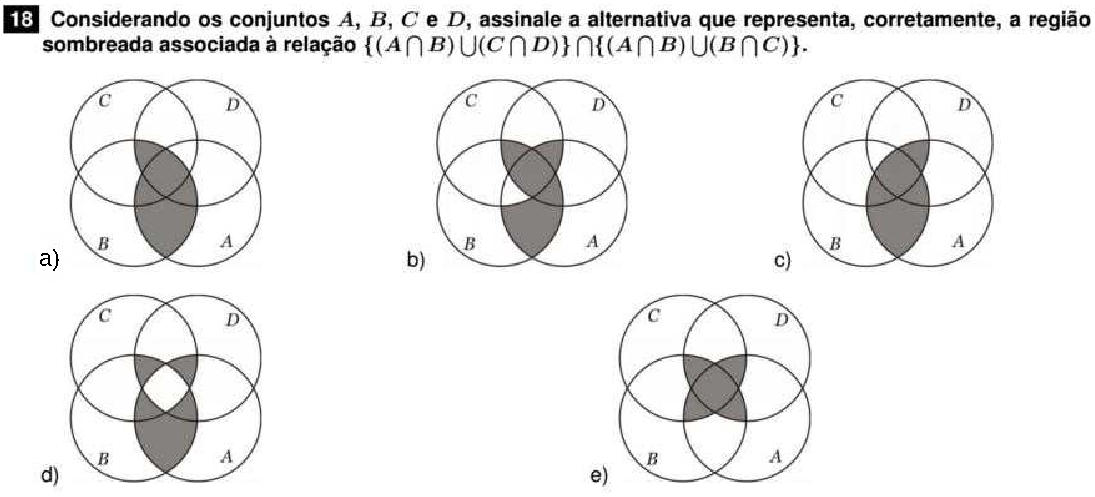
\includegraphics[width=0.9\textwidth]{./Figs/poscomp18-cropped.pdf}
\end{figure}


\begin{resp}~


    a
\end{resp}


\end{questions}

\newpage

\newpage

\vspace{1cm}
\begin{center}
  \section*{Gabarito}
\end{center}
\Closesolutionfile{ans}% finaliza a gravação das respostas
\begin{Gabarito}{1}
~
        \begin{multicols}{4}
        \begin{enumerate}[a)]
            \item Finito
            \item Infinito
            \item Finito
            \item Infinito
        \end{enumerate}
    \end{multicols}

    
\end{Gabarito}
\begin{Gabarito}{2}
~
    \begin{multicols}{2}
    \begin{enumerate}[a)]
        \item $A = \{ 4, 5, 6, 7\}$
        \item $B = \{ Abril, Junho, Setembro, Novembro \}$
        \item $C = \{Bras\acute{i}lia\}$
        \item $D = \{ 0, 1, 8\}$
        \item $E = \{0, 1, 2, ...\}$
        \item $F = \{ 0 \}$
        \item $A = \{ 5, 6, 7, ...\}$
        \item $B = \{ 3, 4, 5\}$
    \end{enumerate}
\end{multicols}

\end{Gabarito}
\begin{Gabarito}{3}
~

    \begin{enumerate}[a)]
        \item

        \begin{itemize}
                \item $2 \in A$
                \item Se $n \in A$, então $n^2 \in A$
            \end{itemize}

        \item

            \begin{itemize}
                    \item $a_1 = 1$
                    \item $n \in \mathbb{N+}, a_{n+1} = a_{n} + 2n - 1$
                \end{itemize}

        \item

        \begin{itemize}
                \item $1 \in C$
                \item Se $n \in C$, então $3n \in C$
            \end{itemize}
    \end{enumerate}
\end{Gabarito}
\begin{Gabarito}{4}
~

    \begin{multicols}{4}
        \begin{enumerate}[a)]
            \item V
            \item V
            \item F
            \item V
            \item V
            \item F
            \item F (Operador $\in$ é aplicado a elementos e não a conjuntos)
            \item V
            \item V
            \item F (observar operador)
            \item F
            \item V
        \end{enumerate}
      \end{multicols}
\end{Gabarito}
\begin{Gabarito}{5}
~

    Seja $x \in A$. Então $x \in \mathbb{R}$ e $x^2 - 4x + 3 = 0$ ou $(x - 1)(x - 3) = 0$, o que nos dá $x = 1$ ou $x = 3$. Em qualquer dos casos, $x \in \mathbb{N}$ e $1 \leq x \leq 4$, de modo que $x \in B$. Portanto, $A \subseteq B$. O número 4 pertence a B, mas não pertence a A, logo $A \subset B$.
\end{Gabarito}
\begin{Gabarito}{6}
~

    Sejam $A = \{x | x \in x^2 < 15\}$ e $B = {x | x \in \mathbb{N} e 2x < 7}$.

    Para provar que $A = B$, vamos mostrar que $A \subseteq B$ e $B \subseteq A$. Para $A \subseteq B$, precisamos escolher um elemento arbitrário de A — ou seja, qualquer coisa que satisfaça a propriedade que caracteriza os elementos de A — e mostrar que satisfaz a propriedade que caracteriza os elementos de B. Seja $x \in A$. Então $x$ é um inteiro não negativo que satisfaz a desigualdade $x^2 < 15$. Os inteiros não negativos cujos quadrados são menores do que 15 são 0, 1, 2 e 3, logo esses são os elementos de A. O dobro de cada um desses inteiros não negativos é um número menor do que 7. Portanto, todo elemento de A pertence a B e $A \subseteq B$.

    Vamos mostrar agora que $B \subseteq A$. Todo elemento de B é um inteiro não negativo cujo dobro é menor do que 7. Esses números são 0, 1, 2 e 3, e cada um deles tem o quadrado menor do que 15, logo $B \subseteq A$.
\end{Gabarito}
\begin{Gabarito}{7}
~

    $\wp(A) = \{\emptyset, \{1\}, \{2\}, \{3\}, \{1, 2\}, \{1, 3\}, \{2, 3\}, \{1, 2, 3\}\}$.
\end{Gabarito}
\begin{Gabarito}{8}
~

    $2^n$ elementos.
\end{Gabarito}
\begin{Gabarito}{9}
~

    c
\end{Gabarito}
\begin{Gabarito}{10}
~

    \begin{multicols}{2}
    \begin{enumerate}[a)]
        \item - (anulada) [$A \cup B = \mathbb{N}$]
        \item F
        \item V
        \item - (anulada) [$A \cup C = A$]
        \item V
    \end{enumerate}
\end{multicols}
\end{Gabarito}
\begin{Gabarito}{11}
~

    \begin{multicols}{2}
    \begin{enumerate}[a)]
        \item 10
        \item $\{1,2,3,4,5,7,8,9,10\}$
        \item $\{ 1,2,3 \}$
        \item $\{ 2,8 \}$
        \item $\{ 1,2,3,4,6,7,9 \}$
    \end{enumerate}
\end{multicols}
\end{Gabarito}
\begin{Gabarito}{12}
~

    \begin{multicols}{2}
        \begin{itemize}
            \item $[(A \cup B) \cap C] \cup \left[(A \cup B) \cap \overline{C} \right]$
            \item $(A \cup B) \cap (C \cup \overline{C})$
            \item $(A \cup B) \cap S$
            \item $(A \cup B)$
        \end{itemize}

        \begin{itemize}
            \item (comutatividade)
            \item (distributividade)
            \item (complemento)
            \item (elemento neutro)
        \end{itemize}
    \end{multicols}
\end{Gabarito}
\begin{Gabarito}{13}
~

    $[C \cup (A \cap B)] \cap \left[(A \cap B) \cup \overline{C}\right] = A \cap B$

\end{Gabarito}
\begin{Gabarito}{14}
~

    \begin{multicols}{2}
        \begin{itemize}
            \item $A \cup (B \cap \overline{B})$
            \item $A \cup \emptyset$
            \item $A$
        \end{itemize}

        \begin{itemize}
            \item (distributividade)
            \item (complemento)
            \item (elemento neutro)
        \end{itemize}
    \end{multicols}
\end{Gabarito}
\begin{Gabarito}{15}
~
    \begin{enumerate}[a)]
        \item $\{ -1, 1 \}$
        \item $\{ -3, -2, -1, 0, 1, 2, 3 \}$
        \item $\{{4,8,12,16,20,...} \}$
    \end{enumerate}

\end{Gabarito}
\begin{Gabarito}{16}
~

    \begin{enumerate}[a)]
        \item $\{ x | (\exists y)( y \in \{1,2,3,4\} ~ e ~ x = y^2) \}$
        \item $\{ x | \text{x são os números primos}\}$
        \item $\{{x| \text{x é um inteiro não negativo escrito em forma binária}}\}$
    \end{enumerate}

\end{Gabarito}
\begin{Gabarito}{17}
~

    \begin{center}
        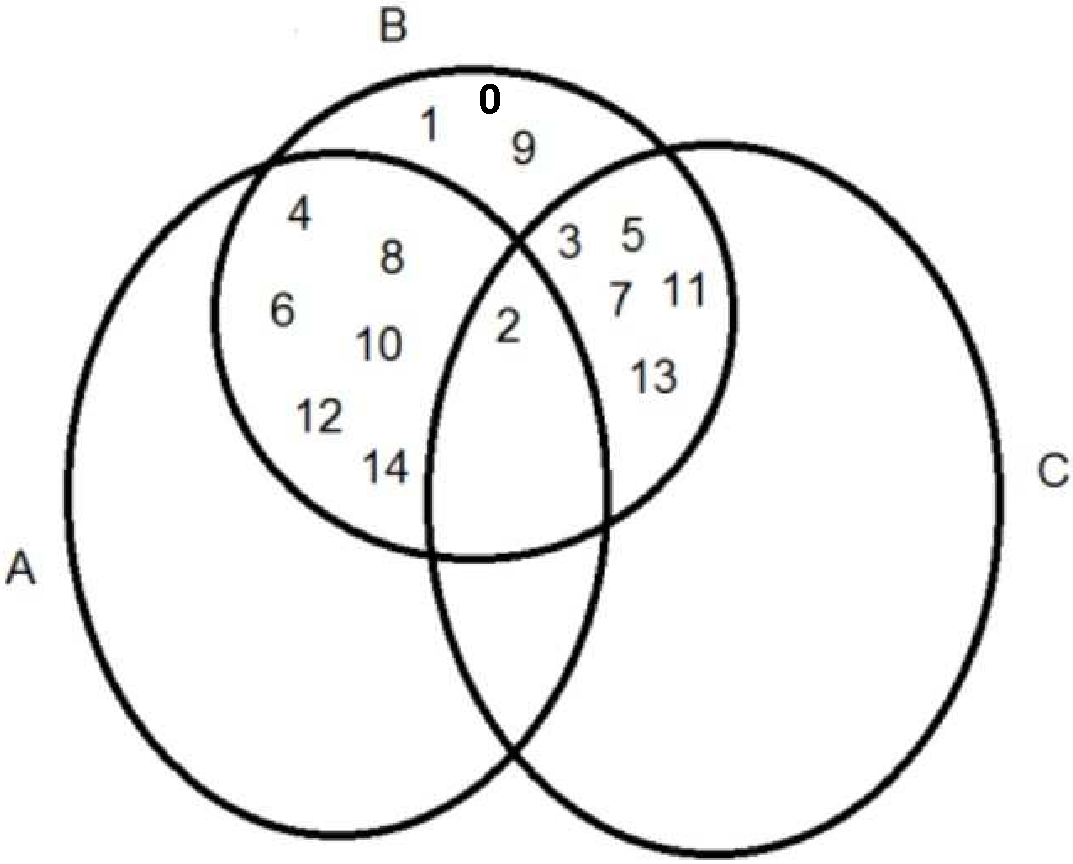
\includegraphics[width=.4\linewidth]{Figs/conjuntos-cropped.pdf}
    \end{center}

\end{Gabarito}
\begin{Gabarito}{18}
~

    \begin{center}
        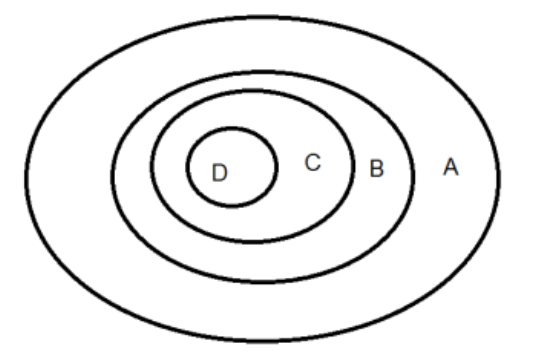
\includegraphics[width=.4\linewidth]{Figs/conjuntos2.png}
    \end{center}
\end{Gabarito}
\begin{Gabarito}{19}
~

    \begin{multicols}{2}
    \begin{enumerate}[a)]
        \item $\{1,2,3,4,5\}$
        \item $\{1,3\}$
        \item $\{5,7,9,11,...\}$
        \item $\{0,5,6,7,8,9,11,13,15,17,...\}$
        \item $\{ 4, 2, \infty\}$
    \end{enumerate}
\end{multicols}

\end{Gabarito}
\begin{Gabarito}{20}
~

    \begin{enumerate}[a)]
        \item $\{(a,x),(a,y),(b,x),(b,y),(c,x),(c,y)\}$
        \item $\{(0,a),(0,b),(0,c),(1,a),(1,b),(1,c)\}$
    \end{enumerate}
\end{Gabarito}
\begin{Gabarito}{21}
~

    \begin{enumerate}[a)]
    \item
    \begin{multicols}{2}
        \begin{itemize}
            \item $A \cup (B \cap \overline{B})$
            \item $A \cup \emptyset$
            \item $A$
        \end{itemize}

        \begin{itemize}
            \item (distributividade)
            \item (complemento)
            \item (elemento neutro)
        \end{itemize}
    \end{multicols}

    \item

    Correção: $A \cap (B \cup \overline{A}) = B \cap A$

    \begin{multicols}{2}
        \begin{itemize}
            \item $(A \cap B) \cup (A \cap \overline{A})$
            \item $(A \cap B) \cup \emptyset$
            \item $(A \cap B)$
            \item $(B \cap A)$
        \end{itemize}

        \begin{itemize}
            \item (distributividade)
            \item (complemento)
            \item (elemento neutro)
            \item (comutatividade)
        \end{itemize}
    \end{multicols}
\end{enumerate}
\end{Gabarito}
\begin{Gabarito}{22}
~

    $A=\{1,3,5,6,7,8,9\}$ e $B=\{2,3,6,9,10\}$
\end{Gabarito}
\begin{Gabarito}{23}
~

    $X=\{1,3,5\}$
\end{Gabarito}
\begin{Gabarito}{24}
~


    a
\end{Gabarito}
 %imprime as soluções
\end{document}
